Por exemplo, considere um projeto de um \textit{software} militar com alta configuração, alta performance, 
com processamento bastante complexo e com bastantes requisitos de segurança, porém com baixa transação de dados.
Considere também que os demais fatores são baixos e que o \textit{backlog} deste projeto 
contabilize 25 \textit{Story Points} e que o \textit{velocity} do time seja 10 pontos/\textit{sprint}.

Considerando uma série quadrada para a escala, teríamos os dados ilustrados pela Figura \ref{example-data}.

  \begin{figure}[!htb]
    \centering
    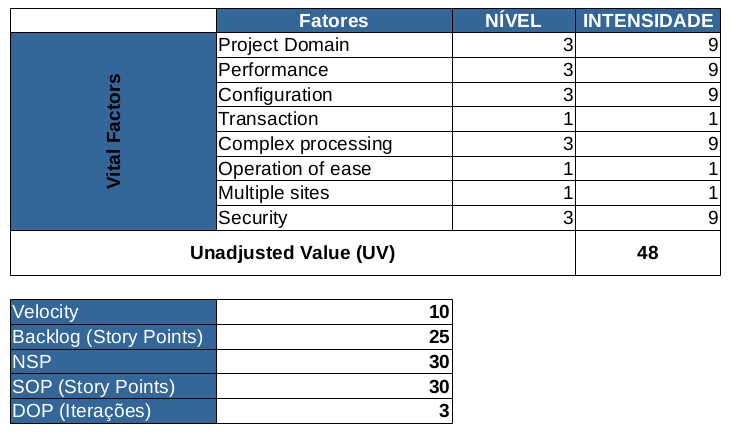
\includegraphics[scale=0.55]{figuras/example-data}
    \caption{Dados da estimativa para o exemplo.}
    \label{example-data}
  \end{figure}
  
Utilizando a técnica apresentada, temos que o tamanho do projeto ficou 5 pontos maior do que era antes de aplicar a técnica,
o que mostra que considerando os fatores do projeto na estimativa pode se obter uma estimativa mais realista.

Consequentemente, conseguimos calcular a duração do projeto a partir do \textit{velocity} informado, que resultou em 3 
iterações para cumprir o \textit{backlog} inicial. Considerando que o \textit{velocity} informado foi calculado utilizando
uma iteração de 2 semanas, temos que o projeto duraria 6 semanas.


